
\documentclass[t,compress,11pt,xcolor=dvipsnames]{beamer}
\usefonttheme[onlymath]{serif}
\definecolor{LHCblue}{RGB}{4, 114, 255}
\usecolortheme[named=LHCblue]{structure}
\usepackage[bars]{beamerthemetree} % Beamer theme v 2.2
\usepackage{multicol}
\usepackage{lmodern}
\usepackage{lipsum}
\usepackage{marvosym}
\title{ CS251 Project Report by Group 04.}
\author{
Mridul Sayana\\
\texttt{140050001}\\
\texttt{140050001@iitb.ac.in}\\
\and
Surender Singh Lamba\\
\texttt{140050075}\\
\texttt{140050075@iitb.ac.in}\\
\and
Thanuj Raju\\
\texttt{140050077}\\
\texttt{140050077@iitb.ac.in}
}
\begin{document}
\maketitle
\begin{frame}
\frametitle{Overview}
\tableofcontents
\end{frame}
\section{Introduction}
\begin{frame}
%\frametitle{Introduction}
This report is made to describe the concepts behind our CS251 project Box2d simulation .\\~\\
We also would like to mention the references used to complete our project through this report.\\~\\
\end{frame}
%
\section{Motivation}
\begin{frame}
\frametitle{Motivation}
This project is a demonstration of the power of the software
systems like BOX2d .\\~\\

 The basic concepts and machinery used in this can be utilized to generate even more complex and relevant games.\\~\\

So we wish to build a machine which explores the whole power of Box2d and demonstrates it visually!\\~\
This project involves several concepts discussed in this course like
makefile, doxygen, bash, beamer, libraries,html etc...\\~\\
This serves as a good and brief outlook of this course.\\~\\
\end{frame}
\section{ Base Code Problems}
\begin{frame}
\frametitle{Base Code Problems}
The crux of our simulation is the water and representing it with a bunch of balls is not doing justice to simulation and also effects RAM very badly.\\~\\

So, while searching for an effective way for this, we stumbled upon LiquidFun which is an extension of Box2D and has a particle module which efficiently does the task we want. \\~\\

For the documentation of LiquidFun, you can visit their github page at http://google.github.io/liquidfun/  \\~\\
\begin{center}

\includegraphics[width=50px,height=50px]{liq.png}
\end{center}

\end{frame}
\begin{frame}
\frametitle{Base Code Problems}
We have used Box2D version 2.3.0, a different base code from the one provided to us. Well, Desperate times, Desperate measures. \\~\\
LiquidFun is a 2D rigid-body and fluid simulation C++ library for games based upon Box2D. It provides support for procedural animation of physical bodies to make objects move and interact in realistic ways.\\~\\
This version has direct support with ios, android, cocos, javascript and vbx\\~\\
\end{frame}
\section{Description}
\frametitle{Description}
\begin{frame}
\begin{center}
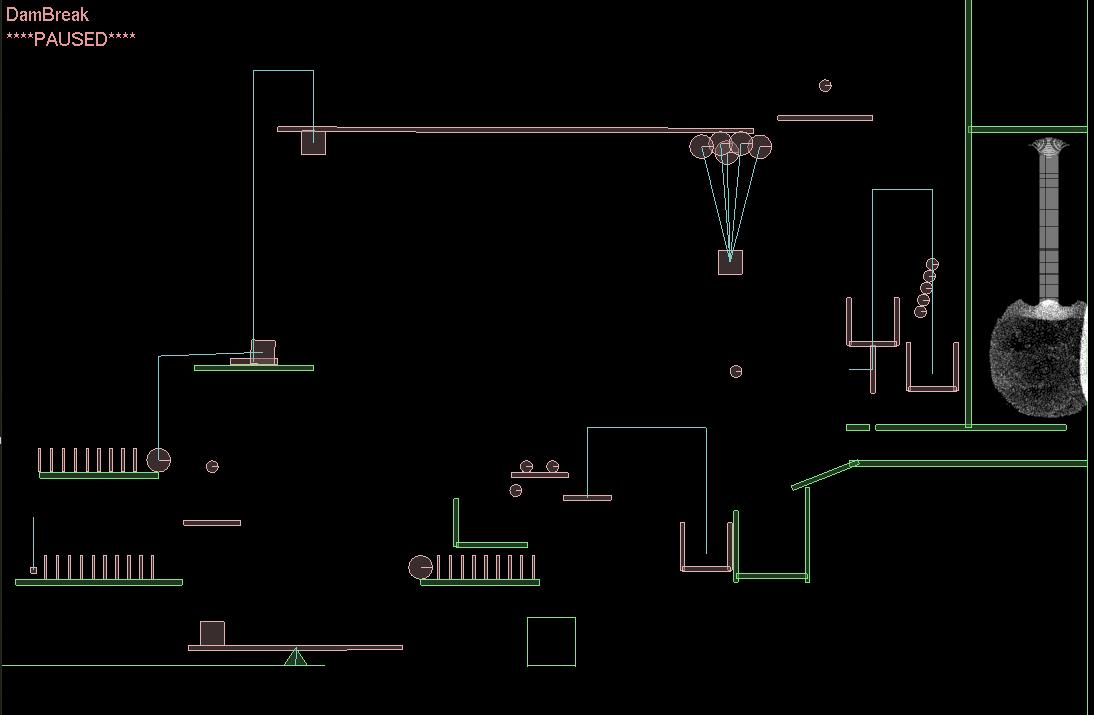
\includegraphics[width=12cm,height=6cm]{Selection_002}
\end{center}
Outlook our our simulation which involves different physics concepts\\~\\
\end{frame}
\begin{frame}
\frametitle{FLUID}
\begin{center}
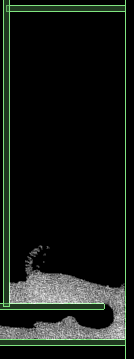
\includegraphics[width=5cm,height=4cm]{liquid}
\end{center}
We found difficult to create Liquid using our Box2D so we used extended version of our Box2D  includes LiquidFun which can create liquid.\\~\\
\end{frame}
\begin{frame}
\frametitle{COMMON BALANCE}
\begin{center}
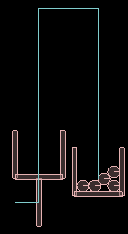
\includegraphics[width=5cm,height=4cm]{balancing}
\end{center}
We used pulley joints to make this balance.\\~\\
It takes two anchors and two objects and connects the two objects with
the thread through two points giving the effect of a common balance.\\~\\
\end{frame}
\begin{frame}
\frametitle{DOMINOS}
\begin{columns}[t]
\column{0.5\textwidth}
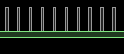
\includegraphics[width=5cm,height=4cm]{dominos}
\column{0.5\textwidth}
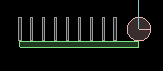
\includegraphics[width=5cm,height=4cm]{dominos_2}
\end{columns}
We made it by placing a static platform and placing a small  dynamic rectangular blocks at regular intervals in such a way that if one of then falls remaining dominos will fall
\end{frame}
\begin{frame}
\frametitle{SEE-SAW}
\begin{columns}[t]
\column{0.5\textwidth}
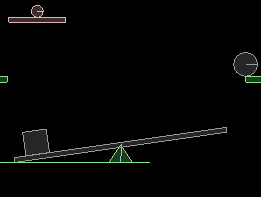
\includegraphics[width=5cm,height=4cm]{see-saw_1}
\column{0.5\textwidth}
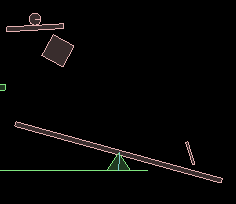
\includegraphics[width=5cm,height=4cm]{see-saw}
\end{columns}
We made the simulation by creating a revolute joint between a static triangle and a dynamic rod,and placing a rectangular block on the plank\\~\\
We arranged the system such that after ball hitting the other side of see-saw that block hits the hinged platform above it.
\end{frame}
\begin{frame}
\frametitle{REVOLVING PLATFORMS}
\begin{center}
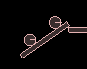
\includegraphics[width=4cm,height=2cm]{hinge}
\end{center}
We used Revolute Joint to make the effect of hinged rod.
It takes one anchors and two objects and connects the two objects with
the thread through the point.\\~\\
We defined one of the objects as a dynamic rod and other as a small
static object with the anchor point on itself which resulted in the effect
of this hinged rod
\end{frame}
\begin{frame}
\frametitle{BALLOONS}
\begin{center}
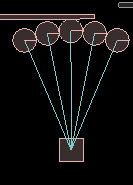
\includegraphics[width=5cm,height=4cm]{balloon}
\end{center}
This is the Balloon system.\\~\\
We made the simulation by changing the gravity of balloon to negative.\\~\\
\end{frame}
\begin{frame}
\frametitle{PENDULUM}
\begin{center}
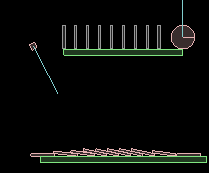
\includegraphics[width=5cm,height=4cm]{pendulum}
\end{center}
It is created using anchoring the thread such that the pendulum hits the dominos above it.
\end{frame}
\section{Profiling}
\begin{frame}
\frametitle{About Profiling}
Profing is very useful to write optimised programs.It gives the description of time consumed by different functions in our code so that we can understand which function to be optimised.\\~\\
The picture in the next slide is very big, so to see clearly, you can see the picture outside in the report folder.
\end{frame}
\begin{frame}
\frametitle{Profiled output of Project}
\begin{center}
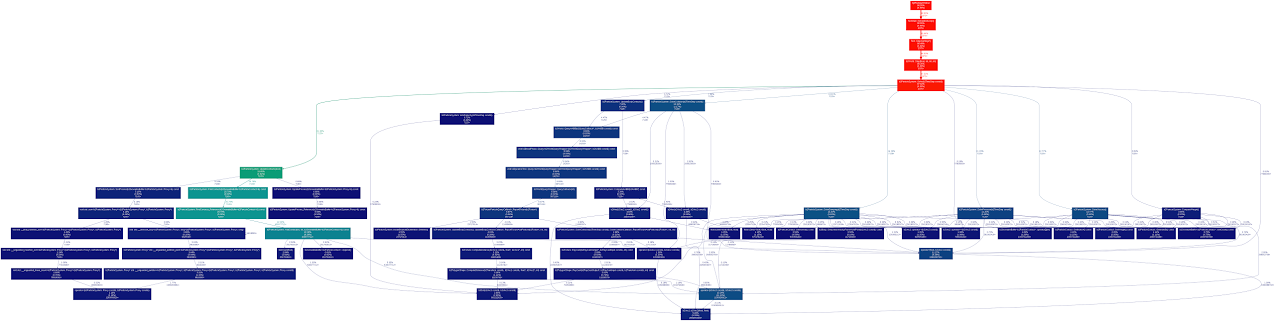
\includegraphics[width=10cm,height=7cm]{gprof}
\end{center}
c\end{frame}
\section{Citations and Thankyous }
\begin{frame}
\frametitle{Citations}
For base code we have used the LiquidFun under Creative Commons license and Copyright (c) 2006-2013 is held by Erin Catto http://www.gphysics.com. Link to github https://github.com/google/liquidfun \\~\\
For the html we have used a template from which is also opensource \\~\\
Credits to Jose Fonseca for gprof2dot.py to make the profiling easy. Link to github https://github.com/jrfonseca/gprof2dot\\~\\
Stack Overflow has been of much help for the project. \\~\\
\end{frame}
\begin{frame}
\frametitle{Thankyous}
This project uses many of the things we learned this semester.\\~\\
Some of the mainly helpful things were cmake, Makefiles, gprof and tex files\\~\\
And as goes with Occams Razor principle, here we officially thank people.\\~\\
Thanks for an informative and exciting semester to Prof.Sharat Chandran and always supportive TA Akash Chaudhary.\\~\\
\end{frame}
\end{document}